\thispagestyle{empty}
\begin{center}
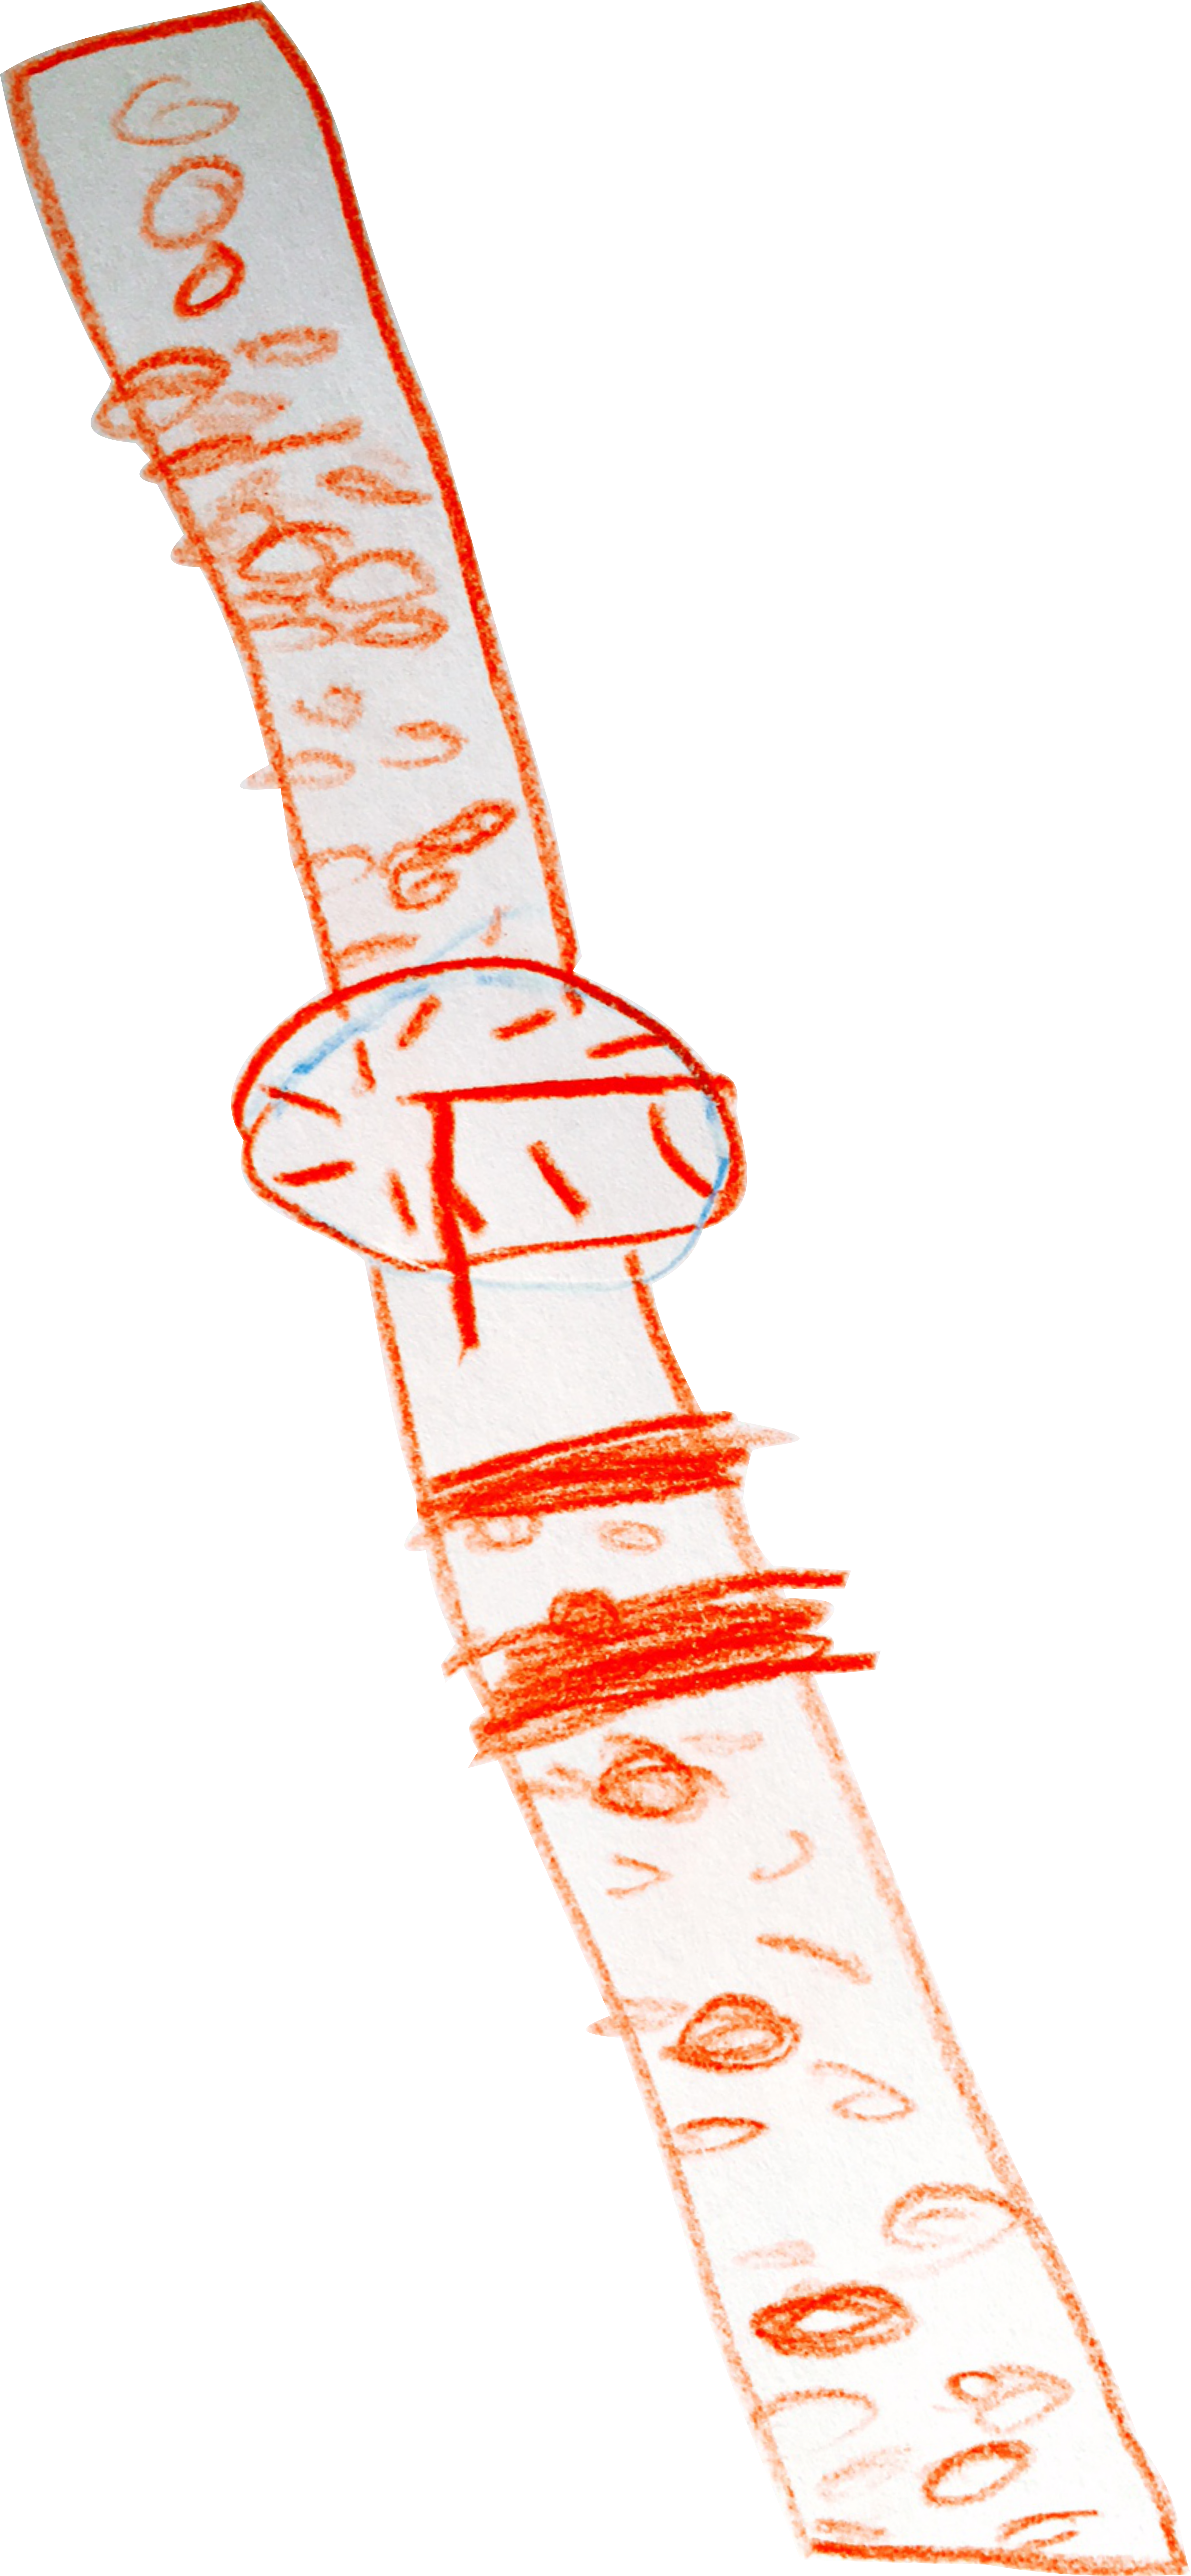
\includegraphics[height=.8\textheight]{./bilder/160120_uhr.png}
\end{center}
\vskip 2cm
{\Huge\color{farbe}\hfill{\tt{Die Wüste}}}
\addcontentsline{toc}{chapter}{Die Wüste}
\newpage
%%%%%%%%%%%%%%%%%%%%%%%%%%%%%%%%%%%%%%%%%%%%%%%%%%%%%%%%%%%%%%%%%%%%%%%%%%%%%%%
\lettrine[lines=2, lhang=.2, loversize=.25, lraise=0.05, findent=0.1em,
nindent=0em]{A}{}ls Thomas Brenton erwachte, lag er alleine mitten in der
Sahara. Die erste Sekunde benötigte er, um wach zu werden. Die zweite um zu
merken, dass er alleine war. Die Karavane, mit er gekommen war, war
verschwunden. Dann kam die Panik, schreien, suchen. 

Nachdem Thomas die Panik einigermassen kontrollieren konnte und noch bevor die
Verzweiflung begann, durchsuchte er sein Bündel nach etwas zu Essen, aber vor
allem nach Wasser. Aber das einzige, was er fand, war ein Zettel auf dem
geschrieben stand: \enquote{Willkommen in deinem Land, König Thomas}

-----

Ein Jahr zuvor. 



\vfill
